\documentclass[12pt, a4paper, reqno, oneside]{book}
\usepackage[left=2.5cm, right=2cm, top=2cm, bottom=2cm]{geometry}
\usepackage{amsmath,amssymb,amsfonts,amsthm}
\usepackage{microtype}
\usepackage{indentfirst}
\usepackage[USenglish]{babel}
\usepackage{graphicx}
\usepackage{float}
\usepackage{listings}
\usepackage[dvipsnames]{xcolor}
\usepackage{tikz}
\usetikzlibrary{calc}
\usepackage{array}
\usepackage{titlesec}
\usepackage{fancyhdr}
\usepackage{tabularx}
\usepackage[square,numbers]{natbib}
\usepackage[labelfont=bf, textfont=it, justification=centering]{caption}
\usepackage{booktabs}
\fancyhf{}
\fancyhead[L]{\small{\leftmark}}
\fancyfoot[C]{ \thepage}
\setlength{\headheight}{14pt}
\captionsetup{labelfont={color=blue, bf}, textfont={color=black, it}}

\usepackage[colorlinks,bookmarksopen,bookmarksnumbered,citecolor=blue, colorlinks=true,linkcolor=blue,urlcolor=blue]{hyperref}

\renewcommand{\baselinestretch}{1.25}

\newcommand \chap[1]{%
  \chapter*{#1}%
  \phantomsection%
  \addcontentsline{toc}{chapter}{#1}
  \markboth{#1}{}
}
\newcommand \sect[1]{%
  \section*{#1}%
  \phantomsection%
  \addcontentsline{toc}{section}{#1}}
  

\renewcommand{\theequation}{\arabic{chapter}.\arabic{equation}} %\arabic{section}.
\newtheorem{lemma}{\bf Bổ đề}[chapter]
\newtheorem{theorem}{\bf Định lý}[chapter]
\newtheorem{proposition}{\bf Mệnh đề}[chapter]
\newtheorem{corollary}{\bf Hệ quả}[chapter]
\newtheorem{definition}{\bf Định nghĩa}[chapter]
\newtheorem{remark}{\bf Chú ý}[section]
% \newtheorem{problem}{Bài toán}
% \renewcommand*{\listalgorithmcfname}{List of Algorithms}
% \renewcommand*{\algorithmcfname}{Algorithm}
% \renewcommand*{\algorithmautorefname}{thuật toán}

%mức tiêu đề
\titleclass{\subsubsubsection}{straight}[\subsection]

\newcounter{subsubsubsection}[subsubsection]
\renewcommand\thesubsubsubsection{\thesubsubsection.\arabic{subsubsubsection}}
\renewcommand\theparagraph{\thesubsubsubsection.\arabic{paragraph}} % optional; useful if paragraphs are to be numbered

\titleformat{\subsubsubsection}
  {\normalfont\normalsize\bfseries}{\thesubsubsubsection}{1em}{}
\titlespacing*{\subsubsubsection}
{0pt}{3.25ex plus 1ex minus .2ex}{1.5ex plus .2ex}

\makeatletter
\renewcommand\paragraph{\@startsection{paragraph}{5}{\z@}%
  {3.25ex \@plus1ex \@minus.2ex}%
  {-1em}%
  {\normalfont\normalsize\bfseries}}
\renewcommand\subparagraph{\@startsection{subparagraph}{6}{\parindent}%
  {3.25ex \@plus1ex \@minus .2ex}%
  {-1em}%
  {\normalfont\normalsize\bfseries}}
\def\toclevel@subsubsubsection{4}
\def\toclevel@paragraph{5}
\def\toclevel@paragraph{6}
\def\l@subsubsubsection{\@dottedtocline{4}{7em}{4em}}
\def\l@paragraph{\@dottedtocline{5}{10em}{5em}}
\def\l@subparagraph{\@dottedtocline{6}{14em}{6em}}
\makeatother

\setcounter{secnumdepth}{4}
\setcounter{tocdepth}{4}


%thư mục hình
\graphicspath{{./figs/}}

\definecolor{mygreen}{rgb}{0,0.6,0}
\definecolor{mygray}{rgb}{0.5,0.5,0.5}
\definecolor{mymauve}{rgb}{0.58,0,0.82}

\lstdefinestyle{customc}{
  belowcaptionskip=1\baselineskip,
  breaklines=true,
  frame=single,
  xleftmargin=\parindent,
  language=C,
  showstringspaces=false,
  basicstyle=\footnotesize\ttfamily,
  keywordstyle=\bfseries\color{green!40!black},
  commentstyle=\itshape\color{purple!40!black},
  identifierstyle=\color{blue},
  stringstyle=\color{orange},
  numbers=left,                   % where to put the line-numbers
  numberstyle=\tiny\color{gray},  % the style that is used for the line-numbers
  stepnumber=1, 
}

\lstdefinestyle{customasm}{
  belowcaptionskip=1\baselineskip,
  frame=single,
  xleftmargin=\parindent,
  language=[x86masm]Assembler,
  basicstyle=\footnotesize\ttfamily,
  commentstyle=\itshape\color{purple!40!black},
  numbers=left,                   % where to put the line-numbers
  numberstyle=\tiny\color{gray},  % the style that is used for the line-numbers
  stepnumber=1, 
}

\lstset{escapechar=@,style=customc}

\definecolor {processblue}{cmyk}{0.96,0,0,0}

\newcolumntype{C}[1]{>{\centering\arraybackslash}p{#1}}

\definecolor{eclipseStrings}{RGB}{42,0.0,255}

\definecolor{eclipseKeywords}{RGB}{127,0,85}

\colorlet{numb}{magenta!60!black}



\lstdefinelanguage{json}{
    basicstyle=\normalfont\ttfamily,
    commentstyle=\color{eclipseStrings}, % style of comment
    stringstyle=\color{eclipseKeywords}, % style of strings
    numbers=left,
    numberstyle=\scriptsize,
    stepnumber=1,
    numbersep=8pt,
    showstringspaces=false,
    breaklines=true,
    frame=lines,
    string=[s]{"}{"},
    comment=[l]{:\ "},
    morecomment=[l]{:"},
    literate=
        *{0}{{{\color{numb}0}}}{1}
         {1}{{{\color{numb}1}}}{1}
         {2}{{{\color{numb}2}}}{1}
         {3}{{{\color{numb}3}}}{1}
         {4}{{{\color{numb}4}}}{1}
         {5}{{{\color{numb}5}}}{1}
         {6}{{{\color{numb}6}}}{1}
         {7}{{{\color{numb}7}}}{1}
         {8}{{{\color{numb}8}}}{1}
         {9}{{{\color{numb}9}}}{1}
}

\begin{document}
\hypersetup{pageanchor=false}

\begin{titlepage}
\begin{center}
	\begin{tikzpicture}[overlay,remember picture]
	    \draw [line width=3pt,rounded corners=0pt,
	        ]
	        ($ (current page.north west) + (20mm,-20mm) $)
	        rectangle
	        ($ (current page.south east) + (-15mm,20mm) $);
	    \draw [line width=1pt,rounded corners=0pt]
	        ($ (current page.north west) + (21.5mm,-21.5mm) $)
	        rectangle
	        ($ (current page.south east) + (-16.5mm,21.5mm) $);
	\end{tikzpicture}
	\\[1mm]
    \centerline{\bf VIETNAM NATIONAL UNIVERSITY HANOI}
    \centerline{\bf UNIVERSITY OF ENGINEERING AND TECHNOLOGY}
    
    \vspace*{1.8cm}
    \large
        \begin{figure}[H]
        \centering
        
\includegraphics[width=0.23\linewidth]{figs/uet.jpg}
        \end{figure}
    \vspace*{1cm}
    \centerline{\bf VU TIEN TUAN TRUNG}
    \vspace*{2.5cm}
    \centerline{\bf Vehicle-Agnostic Representation Learning }
    \centerline{\bf for Cross-Vehicle CAN Bus }
    \centerline{\bf Intrusion Detection}
    \vspace*{2.5cm}
    \centerline{\bf GRADUATION THESIS}
    \vspace*{0.2cm}
    \centerline{\bf Major: Information Systems}
    
    \vfill
    \centerline{\bf Hanoi - 2026}
    \vspace{13pt}
\end{center}
\end{titlepage}

\newpage

\begin{titlepage}
\begin{center}
	\begin{tikzpicture}[overlay,remember picture]
	    \draw [line width=3pt,rounded corners=0pt,
	        ]
	        ($ (current page.north west) + (20mm,-20mm) $)
	        rectangle
	        ($ (current page.south east) + (-15mm,20mm) $);
	    \draw [line width=1pt,rounded corners=0pt]
	        ($ (current page.north west) + (21.5mm,-21.5mm) $)
	        rectangle
	        ($ (current page.south east) + (-16.5mm,21.5mm) $);
	\end{tikzpicture}
	\\[1mm]
    \centerline{\bf VIETNAM NATIONAL UNIVERSITY HANOI}
    \centerline{\bf UNIVERSITY OF ENGINEERING AND TECHNOLOGY}
    \vspace*{1.8cm}
    \large
        \begin{figure}[H]
        \centering
        
\includegraphics[width=0.23\linewidth]{figs/uet.jpg}
        \end{figure}
    \vspace*{0.9cm}
    \large
    \centerline{\bf VU TIEN TUAN TRUNG}
    \vspace*{2.2cm}
    \centerline{\bf Vehicle-Agnostic Representation Learning }
    \centerline{\bf for Cross-Vehicle CAN Bus }
    \centerline{\bf Intrusion Detection}
    \vspace*{1.7cm}
    \centerline{\bf Major: Information Systems}
    
    \vspace*{1.6cm}
    \centerline{\bf Supervisor: }
    \centerline{\bf Assoc. Prof. Nguyen Ngoc Hoa}
    
    \vfill
    \centerline{\bf Hanoi - 2026}
    \vspace{13pt}
\end{center}
\end{titlepage}



\newpage
\pagenumbering{gobble}
\chapter*{Acknowledgements}
\vspace{20pt}

I would like to express my deepest gratitude to my supervisor, Associate Professor Nguyen Ngoc Hoa, for his invaluable guidance, unwavering support, and continuous encouragement throughout this research. His profound expertise, meticulous feedback, and visionary mentorship were instrumental in navigating the complexities of this study, making the completion of this thesis possible.

AI-assisted tools were used to help organize and draft portions of the prose, refine grammar, and format the document. AI coding assistants also supported syntax suggestions during implementation. The author remains responsible for the research design, experiments, data, code, and conclusions presented in this thesis.

While I have strived for academic rigor, I acknowledge that this research still holds potential for further refinement. I warmly welcome and deeply appreciate any constructive critiques and insights from the examination committee, which will undoubtedly help enhance the quality of this work and guide my future endeavors.

Sincere gratitude!


\newpage
\chapter*{Authorship}
\vspace{20pt}

I declare that this thesis is my original work, conducted under the dedicated supervision of Associate Professor Nguyen Ngoc Hoa. I confirm that this document has not been submitted, either in whole or in part, for any other academic degree or professional qualification at this or any other institution.

All sources, references, and related literature utilized in this study have been comprehensively acknowledged and properly cited. Furthermore, I guarantee that the empirical data and statistical analyses presented herein are the direct results of authentic, independently conducted experiments, ensuring strict methodological rigor and accuracy.

I affirm that this declaration is made with the utmost academic integrity and in full compliance with the academic regulations and policies of the VNU University of Engineering and Technology.

\begin{flushright}
{\it Author}
\hskip 1.5cm\quad


\vskip 2cm
{\bf Vu Tien Tuan Trung }  \quad\ \quad
\end{flushright}
\newpage



\newpage
\chapter*{Abstract}
\vspace{20pt}

Controller Area Network (CAN) intrusion detection systems often report high performance under random or within-vehicle evaluation, yet their reliability may fall when deployed on a different vehicle or exposed to an attack not seen during training. This thesis studies these distribution shifts using the \texttt{can-train-and-test} benchmark and evaluates whether a structural representation can reduce dependence on vehicle-specific CAN identifiers. Traffic is divided into non-overlapping windows of 64 frames and assessed under four zero-shot conditions: known vehicle and attack, unseen vehicle with known attack, known vehicle with unseen attack, and simultaneous vehicle and attack shift. The proposed representation removes globally meaningful CAN-ID bits and combines payload and DLC information with local payload changes, inter-arrival timing, same-ID timing, and within-window identifier and transition statistics. A Transformer encoder is compared with a raw-feature Transformer and a structural XGBoost classifier. In the focused Set~1 experiment, the structural Transformer attains attack F1 scores of 0.9035, 0.9703, 0.7094, and 0.2332 under Conditions A--D, respectively; the raw Transformer scores 0.7649, 0.0002, 0, and 0. The largest observed gain is under known-attack transfer to an unseen vehicle (Condition B). Under the combined shift (Condition D), performance improves over the raw baseline but remains limited, with recall of 0.1322. External experiments show strong results for some DoS and spoofing subsets, alongside substantial failures on OTIDS impersonation and mixed traffic. These findings support structural encoding as a promising way to reduce vehicle-ID dependence, while showing that transfer to unseen attack mechanisms remains unresolved and that broader reproducibility and external validation are needed.

\vspace{1em}
\noindent \textit{\textbf{Keywords:} Controller Area Network, automotive cybersecurity, intrusion detection, cross-vehicle generalization, structural representation, Transformer.}


\newpage
%Table of Contents
\tableofcontents

\newpage
\listoffigures
 

\newpage
\listoftables
% No algorithms are presented in this thesis.

\newpage
\chapter*{List of Abbreviations}
\vspace{20pt}



\begin{table}[H]
\centering
\begin{tabular}{|m{2.5cm}|m{8cm}|}
\hline
AI & Artificial Intelligence \\ \hline
CAN & Controller Area Network \\ \hline
CNN & Convolutional Neural Network \\ \hline
DBC & Database for CAN \\ \hline
DLC & Data Length Code \\ \hline
DoS & Denial of Service \\ \hline
FAR & False Alarm Rate \\ \hline
IDS & Intrusion Detection System \\ \hline
ML & Machine Learning \\ \hline
PR-AUC & Area under the Precision-Recall Curve \\ \hline
XGBoost & eXtreme Gradient Boosting \\ \hline
\end{tabular}
\end{table}




\chap{Introduction}
\label{chap:introduction}
\pagestyle{fancy}
\pagenumbering{arabic}

\sect{Motivation}

Modern vehicles increasingly rely on Controller Area Network (CAN) buses to
exchange messages among electronic control units (ECUs)~\cite{verma2024road}.
The lack of authentication and encryption in the original CAN protocol
~\cite{koscher2010experimental,lampe2023cantrainandtest} makes the bus
vulnerable to injection, replay, denial-of-service, and impersonation
attacks~\cite{checkoway2011comprehensive,verma2024road}. Consequently,
machine-learning-based Intrusion Detection Systems (IDSs) have been
extensively investigated for detecting malicious CAN
traffic~\cite{ghadi2026learning,althunayyan2025survey,song2020dcnn}.

However, a major challenge remains in the generalization of CAN IDSs across
different vehicles. Most learning-based approaches are trained and evaluated
using data collected from the same vehicle or under highly similar data
distributions~\cite{kidmose2025cansleuth,koltai2026canwetrust}. Under such
settings, a model can achieve high detection performance by exploiting
vehicle-specific characteristics of CAN traffic, such as CAN identifier
distributions, message frequencies, transition patterns, and payload
characteristics. These features may be strongly correlated with the vehicle
from which the training data were collected rather than with the underlying
attack behavior~\cite{koltai2026canwetrust,lampe2023cantrainandtest}.

This issue becomes particularly important in practical deployment. An IDS
trained using data from one vehicle should ideally detect attacks on another
vehicle without requiring a complete retraining process. Nevertheless,
changing the vehicle can substantially alter the distribution of CAN traffic.
As a result, a model that performs well under conventional within-vehicle
evaluation may experience a significant performance degradation when
evaluated on an unseen vehicle~\cite{koltai2026canwetrust,kidmose2025cansleuth}.

Therefore, this work focuses on the problem of cross-vehicle generalization
in CAN intrusion detection. Rather than assuming that high within-vehicle
performance indicates a robust IDS, we explicitly evaluate models under
different combinations of vehicle and attack
distributions~\cite{lampe2023cantrainandtest,koltai2026canwetrust}. We first
characterize the degradation of conventional CAN representations under
distribution shifts and then investigate whether a structural representation
of CAN traffic can reduce the dependence on vehicle-specific CAN identifiers
while preserving attack-relevant
information~\cite{khreasat2026relational,meng2023gbids,islam2021ggnb}.

The central motivation of this work is thus to move from learning
vehicle-specific traffic patterns toward learning attack-relevant structural
patterns that are more transferable across
vehicles~\cite{khreasat2026relational}.


\sect{Research Challenges and Research Problem}
Building a CAN IDS that works on unseen vehicles involves several fundamental challenges. In the CAN protocol, each message frame contains a CAN ID, a data payload, and an arrival timestamp \cite{song2020invehicle, lee2017otids}. However, vehicle manufacturers use private database files (DBC) to assign CAN IDs and encode payload signals \cite{lampe2023cantrain, lampe2024curated}. Because of this, two different vehicle models often use different CAN IDs, message frequencies, and payload formats for the same driving function \cite{lampe2024curated}. At the same time, different attacks alter traffic in different ways. Flooding and denial-of-service (DoS) attacks change message timing and ID frequency, while spoofing or masquerade attacks mainly modify payload values or mimic normal message timing \cite{lee2017otids, dupont2019automotive}. Therefore, when an IDS fails on a new dataset, it is difficult to know whether the failure comes from a change in the vehicle, a change in the attack type, or the input features used by the model.

Recent studies have made important progress in CAN intrusion detection, including deep sequence models \cite{song2020invehicle}, time-interval methods \cite{lee2017otids}, transfer learning \cite{tariq2020cantransfer}, and graph-based representations \cite{islam2020graph, meng2023gbids}. In addition, new benchmarks such as can-train-and-test \cite{lampe2023cantrain, lampe2024curated}, CAN-MIRGU \cite{rajapaksha2024canmirgu}, and CICIoV2024 \cite{neto2024ciciov2024} provide diverse traffic for evaluation. Despite this progress, four practical research gaps remain in the current literature:

\textbf{Gap 1 --- Separating vehicle shift from attack shift under zero-shot evaluation.} Many existing CAN IDS studies evaluate models using random or chronological train-test splits from the same vehicle \cite{song2020invehicle, lee2017otids}. Some transfer learning approaches adapt models to new vehicles, but they still require labeled or unlabeled data from the target vehicle for fine-tuning \cite{tariq2020cantransfer}. Although the can-train-and-test benchmark defines four distinct evaluation conditions---known vehicle with known attacks (Condition A), unknown vehicle with known attacks (Condition B), known vehicle with unknown attacks (Condition C), and unknown vehicle with unknown attacks (Condition D) \cite{lampe2023cantrain, lampe2024curated}---few studies systematically compare baseline models across all four conditions. As a result, it remains unclear how much performance degradation is caused by changing the vehicle versus changing the attack type when no target-vehicle retraining is allowed.

\textbf{Gap 2 --- Controlled analysis of feature-group contributions under distribution shifts.} Prior work often assumes that cross-vehicle failure happens mainly because models memorize raw CAN IDs. To avoid this problem, some methods use only message timing \cite{lee2017otids} or only ID transition order \cite{islam2020graph}. However, existing studies rarely conduct a controlled ablation that compares Full features, ID-only, Payload-only, and Timing-only inputs under the exact same cross-vehicle and cross-attack splits. Without this direct comparison, we cannot measure which feature groups provide real attack detection capability, which groups are most sensitive to vehicle changes, and whether removing raw CAN IDs alone is enough to improve generalization.

\textbf{Gap 3 --- Evaluating structural CAN representations and isolating representation gains from model architecture.} Several studies have proposed vehicle-agnostic or graph-based representations that capture relationships between consecutive CAN messages instead of raw ID values \cite{islam2020graph, meng2023gbids}. However, many structural methods ignore payload content to remain independent of vehicle protocols \cite{meng2023gbids}, which limits their ability to detect attacks that alter payload bytes. Furthermore, when recent studies combine new input representations with deep architectures such as Transformers, they often do not separate the effect of the input representation from the effect of the model architecture. A controlled comparison between raw features and structural features---while keeping track of architectural effects---is still needed.

\textbf{Gap 4 --- Testing external generalization and reporting failure boundaries.} Most CAN IDS methods are developed and tested on a single benchmark dataset, such as HCRL \cite{song2020invehicle, lee2017otids} or a single multi-vehicle collection \cite{dupont2019automotive}. Because different datasets use different capture tools, driving conditions, and attack scripts \cite{lampe2024curated, rajapaksha2024canmirgu}, a representation that improves results on one benchmark may not work in the same way on another. Moreover, prior papers mainly report positive detection scores and rarely analyze cases where structural representations fail or perform worse than raw features on specific attack types. Evaluating findings across external datasets \cite{lee2017otids, dupont2019automotive, rajapaksha2024canmirgu, neto2024ciciov2024} within clearly defined experimental scopes---including both improvements and failure cases---remains an important open need.

\sect{Research Objective and Tasks}
\label{sect:objective}
The primary objective of this thesis is to systematically investigate why Controller Area Network (CAN) intrusion detection systems (IDS) degrade under cross-vehicle distribution shifts and to evaluate whether a vehicle-agnostic structural representation can improve zero-shot detection performance on unseen vehicles \cite{lampe2023cantrain, lampe2024curated}. Rather than pursuing a single high F1-score on an isolated train-test split, this study establishes a controlled four-phase empirical framework. The scope of this research encompasses window-level intrusion detection ($W = 64$ consecutive frames) across four zero-shot evaluation conditions (Conditions A, B, C, and D) on the primary \texttt{can-train-and-test} benchmark \cite{lampe2023cantrain, lampe2024curated}, followed by cross-dataset validation on selected subsets of four external benchmarks: \texttt{CAN-MIRGU} \cite{rajapaksha2024canmirgu}, \texttt{CICIoV2024} \cite{neto2024ciciov2024}, \texttt{Automotive CAN Bus Intrusion Dataset v2} \cite{dupont2019automotive}, and \texttt{HCRL OTIDS} \cite{lee2017otids}.

To address the four research gaps, this thesis is guided by the following central research question: \textit{Can a structural representation of CAN traffic improve intrusion detection when the test vehicle is not seen during training?} We decompose this central question into four specific Research Questions (RQ1--RQ4), each mapped directly to a corresponding research gap and experimental phase:

\begin{itemize}
    \item \textit{How does CAN IDS performance change when the test vehicle, the attack type, or both differ from the training conditions under zero-shot evaluation?} \\
    This question aims to quantify and separate the performance degradation caused by changing the vehicle configuration (Condition B) from that caused by encountering novel attack behaviors (Condition C) or simultaneous vehicle and attack shifts (Condition D) \cite{lampe2023cantrain, lampe2024curated}.

    \item \textit{How do CAN ID, payload, and timing feature groups contribute to attack detection capability and cross-vehicle generalization?} \\
    This question investigates which specific input modalities (\textit{Full features}, \textit{ID-only}, \textit{Payload-only}, and \textit{Timing-only}) drive intra-vehicle detection, which groups are most vulnerable to cross-vehicle distribution shifts, and whether simply removing raw CAN IDs is sufficient to preserve transferability \cite{lee2017otids, islam2020graph}.

    \item \textit{Can a 32-dimensional structural representation of CAN traffic reduce dependence on raw vehicle-specific CAN IDs while preserving the payload and timing information needed to detect diverse attack types?} \\
    Furthermore, we examine whether performance improvements under cross-vehicle shifts stem from the structural input representation itself, the deep sequence modeling architecture (Transformer Encoder), or the synergy of both \cite{islam2020graph, meng2023gbids}.

    \item \textit{Do the empirical findings and false-alarm reductions observed on the primary benchmark transfer to independent external CAN datasets, and under which attack scenarios does the structural representation fail?} \\
    This question evaluates the external validity and practical boundaries of our approach across diverse data collection environments without overclaiming universal superiority \cite{dupont2019automotive, rajapaksha2024canmirgu, neto2024ciciov2024}.
\end{itemize}


\sect{Contribution Highlights}
\label{sec:contribution}

This thesis makes four empirical and methodological contributions:
\begin{enumerate}
    \item It frames CAN intrusion detection as a zero-shot transfer problem and uses the four official \texttt{can-train-and-test} conditions to distinguish vehicle shift from attack shift.
    \item It implements a 32-dimensional, frame-level structural representation that excludes raw CAN-ID bits while retaining payload, timing, and local identifier-transition information.
    \item It compares the structural Transformer with both a raw-feature Transformer and a structural XGBoost model using attack-class metrics, PR-AUC, accuracy, and false alarms per 100,000 benign windows. It also audits published benchmark scores using attack-class precision and recall to expose the effect of class imbalance.
    \item It evaluates selected external traffic from four public datasets and reports both successful transfer cases and failure cases, including a marked loss on impersonation traffic.
\end{enumerate}



\newpage

\sect{Thesis Outline}

This thesis is organized into six chapters.

\begin{itemize}
    \item The Introduction presents the cross-vehicle detection problem, research questions, objectives, and contributions.
    \item Chapter~\ref{chap:background} introduces CAN Bus and Intrusion Detection, cross-vehicle and vehicle-agnostic IDS, feature and structure representations, evaluation benchmarks, and the problem formulation.
    
    \item Chapter~\ref{chap:related} reviews conventional CAN IDS features, cross-vehicle transfer, structural representations, and evaluation practice.
    
    \item Chapter~\ref{chap:method} defines the structural feature extractor, Transformer classifier, training protocol, and evaluation metrics.
    
    \item Chapter~\ref{chap:experiments} reports the primary benchmark and external validation results, including their failure boundaries.
    \item Chapter~\ref{chap:conclusions} summarizes the contributions, limitations, and future research directions.
\end{itemize}

The thesis concludes with a summary of contributions, acknowledged limitations and directions for future research.



\chapter{Background}
\label{chap:background}

This chapter introduces the technical fundamentals of the Controller Area Network (CAN) protocol, reviews cross-vehicle intrusion detection, feature representations, and benchmark datasets, and formally defines the problem investigated in this thesis.

\section{CAN Bus and Intrusion Detection}
\label{subsec:can_intrusion_detection}

The Controller Area Network (CAN) is a broadcast serial communication bus designed to connect Electronic Control Units (ECUs) inside modern vehicles \cite{song2020invehicle, lee2017otids}. In a CAN bus network, all ECUs share the same physical transmission medium and communicate by broadcasting message frames. Each standard CAN data frame contains an 11-bit (or 29-bit extended) arbitration identifier (CAN ID), a Data Length Code ($\text{DLC} \in \{0, \dots, 8\}$), and a data payload of up to 8 bytes \cite{lampe2024curated}. Unlike traditional computer networks, CAN frames do not contain source or destination addresses. Instead, the CAN ID serves two purposes: it indicates the type of data contained in the frame and determines bus access priority during bitwise arbitration, where a lower numerical ID value wins priority on the bus \cite{song2020invehicle}.

Because the CAN protocol lacks built-in cryptographic authentication, message encryption, and sender verification, any compromised ECU or external device connected to the On-Board Diagnostics (OBD-II) port can inject malicious frames onto the bus \cite{lee2017otids, dupont2019automotive}. Common in-vehicle cyberattacks are generally grouped into three main categories \cite{song2020invehicle, lee2017otids, dupont2019automotive}:
\begin{itemize}
    \item \textbf{Denial-of-Service (DoS) and Flooding Attacks:} The attacker broadcasts high-priority frames (such as $\text{ID} = \texttt{0x000}$) at a very high rate. Because of priority arbitration, legitimate ECUs cannot access the bus, and the inter-arrival time between consecutive messages drops sharply \cite{song2020invehicle, neto2024ciciov2024}.
    \item \textbf{Fuzzing Attacks:} The attacker injects frames with random or semi-random CAN IDs and payload bytes to trigger unexpected vehicle states. Fuzzing alters both the normal sequence of CAN IDs and the distribution of payload values \cite{lee2017otids, dupont2019automotive}.
    \item \textbf{Spoofing, Impersonation, and Masquerade Attacks:} The attacker transmits frames using a legitimate CAN ID belonging to a target ECU (such as RPM, gear, or wheel speed) while modifying the payload bytes to display false sensor readings or override control commands \cite{song2020invehicle, rajapaksha2024canmirgu, neto2024ciciov2024}. Advanced masquerade attacks also mimic the normal transmission frequency of the target ID, making timing-only detection difficult \cite{dupont2019automotive}.
\end{itemize}

To detect these threats without modifying legacy CAN hardware, researchers have developed Intrusion Detection Systems (IDS) that monitor bus traffic passively \cite{song2020invehicle, lee2017otids}. Existing CAN IDS approaches typically rely on timing and frequency analysis \cite{lee2017otids}, payload signal modeling, message transition matrices \cite{islam2020graph, meng2023gbids}, or deep sequence classifiers such as Convolutional Neural Networks (CNNs) and Long Short-Term Memory (LSTM) networks \cite{song2020invehicle, tariq2020cantransfer}.

\section{Cross-Vehicle and Vehicle-Agnostic IDS}
\label{subsec:cross_vehicle_ids}

A major practical challenge in automotive security is deploying a trained IDS across different vehicle models. Vehicle manufacturers use confidential Database for CAN (DBC) files to define how physical signals map to CAN IDs, transmission periods, and byte layouts \cite{lampe2023cantrain, lampe2024curated}. Consequently, two vehicles from different manufacturers---or even different models from the same manufacturer---exhibit distinct sets of CAN IDs, message frequencies, and payload bit encodings for identical driving functions \cite{lampe2024curated}.

Most early CAN IDS studies evaluate models using train and test splits collected from the same vehicle \cite{song2020invehicle, lee2017otids}. Under this intra-vehicle setting, deep learning models often achieve near-perfect F1-scores because they can easily memorize vehicle-specific CAN ID sequences and static payload patterns \cite{lampe2024curated}. However, when a model trained on one vehicle is tested directly on an unseen vehicle, its performance often drops severely due to distribution shift \cite{lampe2023cantrain, lampe2024curated}.

To address cross-vehicle deployment, two main research directions have emerged. The first direction uses transfer learning, such as CANTransfer \cite{tariq2020cantransfer}, which pre-trains a deep network on a source vehicle and fine-tunes it on labeled data from the target vehicle. While effective, transfer learning still requires collecting data and retraining the model for every new vehicle platform. The second direction seeks zero-shot or vehicle-agnostic detection, where a model trained on source vehicles is applied directly to unseen vehicles without retraining \cite{islam2020graph, lampe2024curated}. In particular, Lampe and Meng introduced the \texttt{can-train-and-test} benchmark \cite{lampe2023cantrain, lampe2024curated} to evaluate models across four combinations of known and unknown vehicles and attacks. Nevertheless, systematic analyses separating performance degradation caused by vehicle shifts from degradation caused by novel attack shifts remain limited.

\section{Feature Groups and Structural Representations}
\label{subsec:feature_structural}

The ability of a CAN IDS to detect attacks and generalize across vehicles depends heavily on its input feature representation. Prior studies generally extract features from three raw modalities:
\begin{enumerate}
    \item \textbf{CAN ID Features:} Sequence models such as Inception-ResNet \cite{song2020invehicle} convert sequences of raw CAN IDs into two-dimensional bit grids. While raw IDs capture normal arbitration order on a single vehicle, they are tied directly to the source vehicle's DBC mapping and fail when the target vehicle uses different hexadecimal IDs \cite{lampe2024curated}.
    \item \textbf{Timing Features:} Interval-based methods \cite{lee2017otids} monitor the time difference between consecutive frames ($\Delta t_{\text{prev}}$) or between frames sharing the same CAN ID ($\Delta t_{\text{same\_ID}}$). Timing features are naturally less dependent on specific hexadecimal ID values and work well against high-rate flooding or DoS attacks. However, timing alone cannot detect payload-modification attacks that preserve normal transmission intervals \cite{dupont2019automotive}.
    \item \textbf{Payload Features:} Payload-based detectors inspect the 8 data bytes of each frame. Raw payload bytes help detect spoofing and fuzzing on a known vehicle, but their bit-level meaning changes across vehicles due to different signal scaling, endianness, and padding rules \cite{lampe2024curated}.
\end{enumerate}

To reduce reliance on raw vehicle-specific CAN IDs, several researchers have proposed structural and graph-based representations \cite{islam2020graph, meng2023gbids}. For example, Islam et al. \cite{islam2020graph} construct message transition graphs from windows of CAN traffic and extract graph properties such as node degree and edge counts. Similarly, Meng et al. \cite{meng2023gbids} propose GB-IDS, which analyzes structural graph features of CAN ID transitions. Although these structural approaches avoid memorizing raw ID values, they face two key limitations. First, pure ID-transition graphs ignore payload dynamics and fine-grained per-frame timing, leaving them blind to attacks that modify payload bytes without breaking the normal ID transition order. Second, existing studies rarely conduct a controlled ablation comparing \textit{Full}, \textit{ID-only}, \textit{Payload-only}, and \textit{Timing-only} feature groups under identical cross-vehicle splits, nor do they isolate whether performance gains come from the structural feature representation or from the underlying deep classifier architecture (such as a Transformer).

\section{Cross-Dataset Evaluation Benchmarks}
\label{subsec:cross_dataset}

Evaluating whether CAN IDS findings generalize beyond a single experimental environment requires testing across diverse datasets. Table~\ref{tab:datasets_overview} summarizes the five public CAN intrusion detection benchmarks used in this thesis:
\begin{itemize}
    \item \textbf{\texttt{can-train-and-test} \cite{lampe2023cantrain, lampe2024curated}:} A curated multi-vehicle dataset designed specifically for cross-vehicle and cross-attack evaluation. It organizes traffic from multiple real vehicles into four distinct evaluation conditions (Conditions A, B, C, and D), making it suitable as our primary benchmark.
    \item \textbf{\texttt{HCRL OTIDS} \cite{lee2017otids}:} A widely used benchmark collected from a Kia Soul vehicle containing DoS, Fuzzy, and Impersonation attack scenarios.
    \item \textbf{\texttt{Automotive CAN Bus Intrusion Dataset v2} \cite{dupont2019automotive}:} A multi-vehicle dataset captured from real cars and a prototype setup, providing diverse driving traces and injection attacks.
    \item \textbf{\texttt{CAN-MIRGU} \cite{rajapaksha2024canmirgu}:} A recent dataset recorded from moving vehicles with real-world benign driving sessions and multiple spoofing and DoS attacks.
    \item \textbf{\texttt{CICIoV2024} \cite{neto2024ciciov2024}:} A realistic Internet-of-Vehicles CAN benchmark featuring benign traffic alongside DoS and spoofing attacks across multiple target signals (such as RPM, speed, steering wheel, and gas).
\end{itemize}

Because these datasets differ in logging hardware, timestamp resolution, driving conditions, and attack injection scripts \cite{dupont2019automotive, lampe2024curated, rajapaksha2024canmirgu}, a representation tuned on one dataset may behave differently on another. Therefore, cross-dataset validation must clearly specify which subsets and attack types are evaluated and report both successful false-alarm reductions and failure cases.

\begin{table}[htbp]
\caption{Overview of Public CAN Intrusion Detection Benchmarks Used in This Thesis}
\label{tab:datasets_overview}
\centering
\renewcommand{\arraystretch}{1.25}
\small
\begin{tabularx}{\textwidth}{p{2.7cm} c p{3.7cm} X}
\hline
\textbf{Dataset} & \textbf{Ref.} & \textbf{Role in This Thesis} & \textbf{Evaluated Traffic and Attack Scope} \\
\hline
\texttt{can-train-and-test} & \cite{lampe2023cantrain, lampe2024curated} & Primary benchmark (Phases 1--3) & Multi-vehicle sets (Set01--Set04) across Conditions A, B, C, and D \\
\texttt{CAN-MIRGU} & \cite{rajapaksha2024canmirgu} & External validation (Phase 4) & Moving-vehicle false-alarm check on selected benign trace (Day 1) \\
\texttt{CICIoV2024} & \cite{neto2024ciciov2024} & External validation (Phase 4) & Benign, DoS, and spoofing scenarios in evaluated test subsets \\
\texttt{Automotive CAN v2} & \cite{dupont2019automotive} & External validation (Phase 4) & Selected vehicles and supported injection attack scenarios \\
\texttt{HCRL OTIDS} & \cite{lee2017otids} & External validation (Phase 4) & DoS, Fuzzy, and Impersonation attack scenarios \\
\hline
\end{tabularx}
\end{table}

\section{Problem Statement and Formulation}
\label{subsec:problem_formulation}

\subsection{CAN Bus Traffic and Windowed Intrusion Detection}
We model the in-vehicle CAN bus traffic generated by a vehicle $v \in \mathcal{V}$ as a continuous, time-ordered stream of message frames $\mathcal{S}^{(v)} = \{F_1, F_2, \dots, F_N\}$ \cite{song2020invehicle, lee2017otids}. Each individual CAN frame $F_i$ is represented as a four-tuple:
\begin{equation}
    F_i = \left( t_i,\, \text{ID}_i,\, \text{DLC}_i,\, \mathbf{b}_i \right),
\end{equation}
where $t_i \in \mathbb{R}_{\ge 0}$ denotes the arrival timestamp in seconds, $\text{ID}_i \in \mathcal{I}^{(v)}$ is the 11-bit or 29-bit arbitration identifier, $\text{DLC}_i \in \{0, 1, \dots, 8\}$ is the Data Length Code specifying the number of active payload bytes $nb_i$, and $\mathbf{b}_i = [b_{i,0}, b_{i,1}, \dots, b_{i,7}] \in \{0, \dots, 255\}^8$ is the 8-byte data payload \cite{lampe2024curated}. Each frame has a ground-truth binary label $y_i \in \{0, 1\}$, where $y_i = 0$ indicates a benign frame and $y_i = 1$ indicates an attack frame.

Because individual CAN frames carry limited context and many attacks manifest through sequential timing and transition anomalies, we formulate intrusion detection at the window level \cite{song2020invehicle, islam2020graph}. The continuous stream $\mathcal{S}^{(v)}$ is partitioned into non-overlapping windows of fixed length $W = 64$ consecutive frames. The $k$-th window $\mathcal{W}_k$ and its binary ground-truth label $Y_k \in \{0, 1\}$ are defined as:
\begin{equation}
    \mathcal{W}_k = \left\{ F_{(k-1)W + 1},\, F_{(k-1)W + 2},\, \dots,\, F_{kW} \right\},
\end{equation}
\begin{equation}
    Y_k = \mathbb{I}\!\left( \sum_{i=(k-1)W+1}^{kW} y_i \ge 1 \right) = 
    \begin{cases} 
        1 & \text{if at least one frame in } \mathcal{W}_k \text{ is malicious}, \\
        0 & \text{otherwise (all frames in } \mathcal{W}_k \text{ are benign)}.
    \end{cases}
\end{equation}

\subsection{Cross-Vehicle Distribution Shift and Four Evaluation Conditions}
Each vehicle model $v$ uses a private DBC specification $\mathcal{M}_v$ that maps physical signals to vehicle-specific arbitration identifiers $\mathcal{I}^{(v)}$, transmission periods, and byte-level payload formats \cite{lampe2023cantrain, lampe2024curated}. Thus, for two different vehicles $v_{\text{train}} \neq v_{\text{test}}$, the traffic distributions differ substantially:
\begin{equation}
    \mathcal{I}^{(v_{\text{train}})} \neq \mathcal{I}^{(v_{\text{test}})} \quad \text{and} \quad P_{v_{\text{train}}}\!\left(\mathcal{W}_k,\, Y_k\right) \neq P_{v_{\text{test}}}\!\left(\mathcal{W}_k,\, Y_k\right).
\end{equation}

Let $\mathcal{V}_{\text{train}}$ and $\mathcal{V}_{\text{test}}$ denote the sets of training and testing vehicles, and let $\mathcal{A}_{\text{train}}$ and $\mathcal{A}_{\text{test}}$ denote the sets of training and testing attack types. Following the \texttt{can-train-and-test} benchmark \cite{lampe2023cantrain, lampe2024curated}, we define four zero-shot evaluation conditions (summarized in Table~\ref{tab:eval_conditions}) where no retraining or fine-tuning on the test vehicle is permitted:
\begin{itemize}
    \item \textbf{Condition A (Known Vehicle, Known Attack):} $\mathcal{V}_{\text{test}} = \mathcal{V}_{\text{train}}$ and $\mathcal{A}_{\text{test}} = \mathcal{A}_{\text{train}}$. This serves as the intra-vehicle baseline.
    \item \textbf{Condition B (Unknown Vehicle, Known Attack):} $\mathcal{V}_{\text{test}} \cap \mathcal{V}_{\text{train}} = \emptyset$ and $\mathcal{A}_{\text{test}} = \mathcal{A}_{\text{train}}$. This isolates the impact of \textit{cross-vehicle shift}.
    \item \textbf{Condition C (Known Vehicle, Unknown Attack):} $\mathcal{V}_{\text{test}} = \mathcal{V}_{\text{train}}$ and $\mathcal{A}_{\text{test}} \cap \mathcal{A}_{\text{train}} = \emptyset$. This isolates the impact of \textit{cross-attack shift}.
    \item \textbf{Condition D (Unknown Vehicle, Unknown Attack):} $\mathcal{V}_{\text{test}} \cap \mathcal{V}_{\text{train}} = \emptyset$ and $\mathcal{A}_{\text{test}} \cap \mathcal{A}_{\text{train}} = \emptyset$. This evaluates combined vehicle and attack shifts.
\end{itemize}

\begin{table}[htbp]
\caption{Taxonomy of the Four Zero-Shot Evaluation Conditions \cite{lampe2023cantrain, lampe2024curated}}
\label{tab:eval_conditions}
\centering
\renewcommand{\arraystretch}{1.25}
\begin{tabularx}{\textwidth}{c c c X}
\hline
\textbf{Cond.} & \textbf{Vehicle} & \textbf{Attack} & \textbf{Evaluated Shift} \\
\hline
\textbf{A} & Known & Known & In-distribution baseline \\
\textbf{B} & Unseen & Known & Cross-vehicle shift \\
\textbf{C} & Known & Unseen & Cross-attack shift \\
\textbf{D} & Unseen & Unseen & Compound vehicle and attack shift \\
\hline
\end{tabularx}
\end{table}

\subsection{Vehicle-Agnostic Representation Learning Objective}
Given a labeled training set $\mathcal{D}_{\text{train}} = \{(\mathcal{W}_k, Y_k)\}_{k=1}^{M_{\text{train}}}$ from source vehicles $\mathcal{V}_{\text{train}}$ under attacks $\mathcal{A}_{\text{train}}$, an intrusion detection model consists of two mappings: (i) a feature representation mapping $\Phi: \mathcal{W}_k \mapsto X_k \in \mathbb{R}^{W \times D}$ that transforms a $W$-frame window into a $D$-dimensional feature sequence, and (ii) a sequence classifier $f_{\theta}: \mathbb{R}^{W \times D} \mapsto [0, 1]$ with parameters $\theta$ that outputs an intrusion probability $p_k = f_{\theta}(\Phi(\mathcal{W}_k))$. A binary prediction is obtained using a decision threshold $\tau \in (0, 1)$ as $\hat{Y}_k = \mathbb{I}(p_k \ge \tau)$.

When a conventional IDS uses a raw feature mapping $\Phi_{\text{raw}}(\mathcal{W}_k)$ containing raw hexadecimal CAN IDs, the classifier $f_{\theta}$ may learn vehicle-specific patterns that fail under distribution shift. Our objective is to design a \textit{vehicle-agnostic structural representation} $\Phi_{\text{struct}}: \mathcal{W}_k \mapsto X_k \in \mathbb{R}^{64 \times 32}$ that removes raw CAN-ID bits while preserving payload dynamics, timing intervals, and local relational ID transitions \cite{islam2020graph, meng2023gbids}. In the reported implementation, parameters $\theta^*$ are learned on $\mathcal{D}_{\text{train}}$ by minimizing cross-entropy $\mathcal{L}_{\text{CE}}$:
\begin{equation}
    \theta^* = \arg\min_{\theta} \frac{1}{|\mathcal{D}_{\text{train}}|} \sum_{(\mathcal{W}_k, Y_k) \in \mathcal{D}_{\text{train}}} \mathcal{L}_{\text{CE}}\!\left( f_{\theta}\!\left(\Phi_{\text{struct}}(\mathcal{W}_k)\right),\, Y_k \right),
\end{equation}
so that the trained detector $f_{\theta^*} \circ \Phi_{\text{struct}}$ can be evaluated zero-shot across Conditions A--D and external datasets $\mathcal{D}_{\text{ext}}$ \cite{lee2017otids, dupont2019automotive, rajapaksha2024canmirgu, neto2024ciciov2024}.

\chapter{Related Work}
\label{chap:related}

\section{Conventional CAN Intrusion Detection}
\label{sec:rw_conventional}
Early CAN IDS research established that attacks can be detected from the temporal regularity of periodic in-vehicle messages. Lee et al. introduced OTIDS and examined timing patterns and remote-frame behavior, while Song et al. used deep convolutional models to learn patterns from CAN identifiers and payload sequences~\cite{lee2017otids,song2020invehicle,song2020dcnn}. These approaches demonstrated that passive monitoring can detect injection and flooding attacks without changes to vehicle ECUs. Their results also illustrate a recurring evaluation risk: when training and testing traffic come from the same vehicle and capture conditions, a model can exploit stable identifiers and message schedules that may not persist on another platform.

Feature engineering has remained central to automotive IDS research. Inter-arrival intervals are informative for DoS and flooding, which alter bus load and message cadence. Payload features can capture value manipulation and fuzzing, and sequences of message identifiers can reveal departures from normal schedules. Each feature family has a different failure mode: timing can be preserved by carefully paced attacks, payload encodings differ across DBCs, and raw identifiers are vehicle-specific.

\section{Cross-Vehicle Transfer and Benchmarking}
\label{sec:rw_transfer}
Transfer learning methods such as CANTransfer adapt a model trained on one source vehicle using target-vehicle data~\cite{tariq2020cantransfer}. This can reduce the cost of building a detector for each platform, but target data and an adaptation procedure remain necessary. This thesis instead studies zero-shot transfer: test traffic is not used to fit model parameters, thresholds, vocabularies, or feature normalizers.

The \texttt{can-train-and-test} dataset was introduced to support controlled experiments across four vehicle platforms and nine attacks. Its organization distinguishes known from unseen vehicles and known from unseen attacks, enabling four conditions rather than a single undifferentiated transfer score~\cite{lampe2023cantrain,lampe2024curated}. This separation matters because vehicle shift and attack shift are not equivalent. A known attack on an unseen vehicle tests transfer of attack cues across platform-specific traffic; a new attack on a familiar vehicle tests whether the model recognizes behavior beyond its training attack set. The compound condition tests both simultaneously.

Recent dataset audits have emphasized that high aggregate scores can obscure poor minority-class detection and that cross-dataset results depend on label provenance, capture boundaries, and preprocessing~\cite{verma2024road,kidmose2025cansleuth,koltai2026canwetrust}. Accordingly, this thesis prioritizes attack-class precision, recall, and F1, reports false alarms on benign windows, and treats each external dataset as a separate experiment rather than pooling incompatible schemas.

\section{Structural and Graph-Based Representations}
\label{sec:rw_structural}
Graph-based CAN IDS methods represent messages and their transitions as nodes and edges, or summarize transition structure within traffic windows~\cite{islam2020graph,meng2023gbids,islam2021ggnb}. Such approaches can reduce direct dependence on a particular hexadecimal ID by emphasizing relationships among messages. They are especially relevant when attacks perturb the order or frequency of recurring identifiers. However, a transition-only representation may discard payload changes that distinguish spoofing or impersonation attacks.

The representation studied here follows the same broad motivation but operates at frame level. It combines payload values and masks, payload differences from the previous message with the same identifier, causal inter-arrival intervals, same-identifier intervals, and normalized local identifier and transition statistics. The identifier itself is used internally to calculate within-window relationships but its raw bit pattern is not supplied to the classifier. This design tests whether structural context can retain useful attack information while reducing the most direct vehicle-specific cue.

\section{Evaluation Metrics and the Present Study}
\label{sec:rw_metrics}
Accuracy and weighted F1 can be dominated by benign traffic when attack windows are rare. A detector that predicts benign for almost every window may therefore appear competitive despite missing nearly all attacks. Precision and recall for the attack class, their harmonic mean (attack F1), and area under the precision-recall curve provide a more direct view of detection quality. False alarms per 100,000 benign windows add an operational measure of alert burden. No single metric fully characterizes a detector: high precision with low recall can miss attacks, while high recall with low precision may overwhelm operators.

This thesis contributes an implementation-level comparison of raw and structural inputs under matched Transformer architecture, together with a structural XGBoost reference. It evaluates all four benchmark conditions and selected external subsets, then interprets the results in light of class balance and scenario coverage. The empirical claim is bounded by the evaluated splits and the current experimental artifacts.

\chapter{Vehicle-Agnostic Representation Learning Framework}
\label{chap:method}

\section{Overview}
\label{sec:method_overview}
The framework has three stages: parse CAN frames into a canonical sequence, split each source file into non-overlapping windows of 64 frames and extract either raw or structural features, then train a binary classifier using source training data only. Evaluation is performed on the official test folders for Conditions A--D and on selected external files. The primary task is window-level classification. A window is labeled as an attack if at least one of its 64 frames is labeled malicious. Windows do not intentionally cross source-file boundaries.

\section{Raw and Structural Feature Representations}
\label{sec:method_features}
The raw baseline has 29 values per frame: 11 CAN-ID bits, normalized DLC, eight payload bytes normalized to $[0,1]$, eight payload-validity masks, and log-scaled time since the preceding frame. The proposed structural representation has 32 values per frame. Table~\ref{tab:struct_features} lists its feature groups. CAN IDs are used as local keys by the extractor to calculate same-ID history and local window statistics, but no globally meaningful identifier value or bit encoding is passed to the classifier.

\begin{table}[htbp]
\centering
\caption{Frame-level structural feature groups}
\label{tab:struct_features}
\renewcommand{\arraystretch}{1.15}
\begin{tabular}{p{3.6cm} c p{7.2cm}}
\hline
\textbf{Feature group} & \textbf{Dimensions} & \textbf{Definition} \\
\hline
DLC, payload, masks & 17 & Normalized DLC; eight normalized payload bytes; eight indicators for bytes within the declared payload length. \\
Same-ID payload change & 9 & Eight absolute byte differences from the previous frame with that identifier, plus a flag indicating whether such a previous frame exists. \\
Timing & 2 & Log-scaled interval from the preceding frame and from the preceding frame with the same identifier. \\
Local identifier statistics & 3 & Within-window identifier frequency, first-occurrence rank, and local re-indexed token, each normalized by window size or unique IDs. \\
Transition statistic & 1 & Frequency of the immediately preceding-to-current local identifier transition within the current window. \\
\hline
Total & 32 & No raw CAN-ID bits are supplied to the model. \\
\hline
\end{tabular}
\end{table}

For payload byte $b_{i,j}$, the feature value is $b_{i,j}/255$. Inter-arrival features use $\log(1 + 1000\min(\Delta t,10))$, with timestamps expressed in seconds. Same-ID payload differences are $|b_{i,j}-b_{q,j}|/255$, where $q$ is the previous frame with the same identifier available to the extractor. Local frequencies and ranks are computed from the 64-frame window. These operations make local rank features invariant to a one-to-one renaming of identifiers within a window; the payload and timing components are not guaranteed to be invariant to changes in driving conditions or signal encoding.

\section{Classifier and Training Procedure}
\label{sec:method_model}
The sequence classifier projects each per-frame vector to a 64-dimensional hidden representation, adds a learned positional embedding, and applies a two-layer Transformer encoder. Each encoder layer has four attention heads, a feed-forward dimension of 128, GELU activation, and dropout of 0.1. Mean pooling over the 64 encoded frame representations feeds a classifier with layer normalization, a 32-unit ReLU layer, and a two-class output layer. The same architecture is used for the 29-dimensional raw input and 32-dimensional structural input, reducing architecture as a confound in this comparison.

The reported notebook implementation trains with cross-entropy, AdamW (learning rate 0.001, weight decay $10^{-4}$), batch size 128, and a cosine learning-rate schedule for ten epochs. Per source file, training reads a bounded number of frames and samples benign windows to limit imbalance; the notebook uses a fixed random seed for that sampling. Structural XGBoost is trained on flattened window features with 100 estimators, maximum depth 6, learning rate 0.1, and random state 42. Structural feature extraction and model fitting use source training traffic. No target test labels are used for fitting. The reported model is trained with cross-entropy alone; the optional contrastive invariance loss mentioned in the earlier project plan is not part of this implementation.

\section{Evaluation Protocol and Measures}
\label{sec:method_eval}
For the focused Set~1 experiment, the model is trained on the designated \texttt{train\_01} folder and evaluated on its four official test folders. Condition A contains a known vehicle and known attack; B contains an unseen vehicle and known attack; C contains a known vehicle and unseen attack; D combines an unseen vehicle and unseen attack. The four conditions are reported separately to expose distinct shift effects. Other result exports in the workspace represent additional runs and are not pooled with this focused experiment.

The primary metrics are attack-class precision, recall, F1, and average precision (reported as PR-AUC), along with accuracy and false positive windows per 100,000 benign windows. For the attack label, $F_1=2PR/(P+R)$; the false alarm rate is $100{,}000\,FP/N_{\mathrm{benign}}$. The evaluated implementation uses the model's two-class prediction for binary metrics. The notebook exports do not include capture-group bootstrap confidence intervals, so reported differences are descriptive point estimates and are not presented as statistically significant effects.

External validation is conducted as selected-scenario transfer using the available dataset adapters. Dataset schemas and logging conventions differ, and not every file contains an equivalent combination of timestamps, labels, and attack categories. External results are therefore interpreted by dataset and scenario, not as a single pooled estimate.



\chapter{Results and Analysis}
\label{chap:experiments}

\section{Primary Benchmark Results}
\label{sec:primary_results}
Table~\ref{tab:phase3_results} reports the focused Set~1 comparison exported by the Phase~3 notebook. The structural Transformer is the strongest of the three models in Conditions A--D. The largest difference is in Condition B: attack F1 rises from 0.0002 for the raw Transformer to 0.9703 for the structural Transformer, with recall 0.9426 and precision 0.9997. Under Condition C, the structural model attains F1 0.7094 while the raw model detects no attack windows. Under Condition D, structural F1 is 0.2332, an absolute gain of 0.2332 over the raw model's zero F1, but recall is only 0.1322. This combined-shift result is an improvement, not evidence that the method reliably detects unknown attacks on unseen vehicles.

\begin{table}[htbp]
\centering
\caption{Focused Set~1 results by zero-shot condition}
\label{tab:phase3_results}
\small
\renewcommand{\arraystretch}{1.15}
\resizebox{\textwidth}{!}{%
\begin{tabular}{llrrrrr}
\hline
\textbf{Condition} & \textbf{Model} & \textbf{Attack F1} & \textbf{Precision} & \textbf{Recall} & \textbf{PR-AUC} & \textbf{FAR/100k} \\
\hline
A & Raw Transformer & 0.7649 & 1.0000 & 0.6194 & 0.8146 & 0.00 \\
A & Structural Transformer & 0.9035 & 1.0000 & 0.8239 & 0.9587 & 0.00 \\
A & Structural XGBoost & 0.7812 & 0.9990 & 0.6414 & 0.8379 & 2.32 \\
\hline
B & Raw Transformer & 0.0002 & 1.0000 & 0.0001 & 0.9505 & 0.00 \\
B & Structural Transformer & 0.9703 & 0.9997 & 0.9426 & 0.9765 & 2.17 \\
B & Structural XGBoost & 0.8902 & 1.0000 & 0.8021 & 0.9594 & 0.00 \\
\hline
C & Raw Transformer & 0.0000 & 0.0000 & 0.0000 & 0.0643 & 0.00 \\
C & Structural Transformer & 0.7094 & 1.0000 & 0.5497 & 0.8807 & 0.00 \\
C & Structural XGBoost & 0.0078 & 0.9444 & 0.0039 & 0.1814 & 1.58 \\
\hline
D & Raw Transformer & 0.0000 & 0.0000 & 0.0000 & 0.0115 & 0.00 \\
D & Structural Transformer & 0.2332 & 0.9892 & 0.1322 & 0.6900 & 1.47 \\
D & Structural XGBoost & 0.0009 & 0.0169 & 0.0005 & 0.2345 & 28.37 \\
\hline
\end{tabular}
}%
\end{table}

The Condition A result does not show a performance penalty for the structural Transformer in this run; its attack F1 exceeds the raw baseline by 0.1386. Structural XGBoost is substantially weaker than the structural Transformer under Conditions C and D, suggesting that the extracted features alone do not guarantee transfer: the sequence model appears to matter in this implementation. This comparison does not isolate all architecture effects because XGBoost is trained on flattened windows and differs in inductive bias and optimization.

The near-zero FAR values must be read alongside recall. In Condition D, the structural model produces few false alerts but also misses most attacks. Condition C has zero observed false alarms in the exported test set and recall 0.5497. These point estimates over the evaluated windows do not establish an operational false-alarm rate in deployment.

\begin{figure}[htbp]
\centering
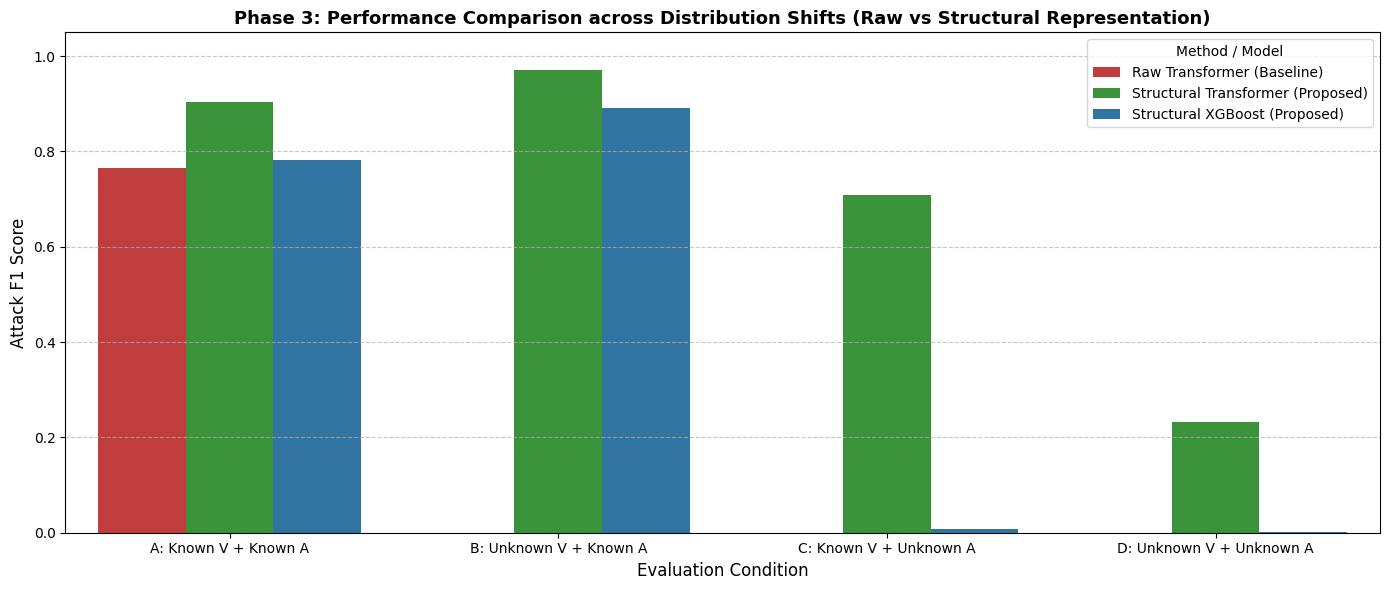
\includegraphics[width=\textwidth]{phase3_benchmark_comparison.png}
\caption{Attack F1 across the four zero-shot conditions in the focused Phase~3 experiment.}
\label{fig:phase3_benchmark}
\end{figure}

Condition B also illustrates the distinction between ranking and classification at a fixed decision rule. The raw Transformer has PR-AUC 0.9505, but attack recall at its exported class decision is 0.0001 and attack F1 is 0.0002. Its scores therefore rank examples favorably according to the reported average-precision calculation while the default class decision yields almost no positive predictions. This mismatch motivates reporting both ranking measures and threshold-dependent operating metrics; it also makes source-only calibration an important follow-up.

\section{Cross-Set Sweep and Reproducibility}
\label{sec:cross_set_sweep}
An additional four-set result export is available in \texttt{master\_all\_datasets\_benchmark.csv}. Table~\ref{tab:multiset_sweep} reports its structural Transformer attack F1 values as a separate exploratory run. Performance varies considerably across sets. The model has high F1 in Conditions A and B on Set~1 and Set~2, but the exported Set~3 values are zero throughout and Set~4 Condition B is 0.3032. These results show that the favorable focused result should not be generalized to all vehicle pairs.

\begin{table}[htbp]
\centering
\caption{Exploratory four-set sweep: structural Transformer attack F1}
\label{tab:multiset_sweep}
\begin{tabular}{lrrrr}
\hline
\textbf{Set} & \textbf{A} & \textbf{B} & \textbf{C} & \textbf{D} \\
\hline
Set~1 & 0.7741 & 0.9635 & 0.0976 & 0.0010 \\
Set~2 & 0.8028 & 0.8476 & 0.9649 & 0.8801 \\
Set~3 & 0.0000 & 0.0000 & 0.0000 & 0.0000 \\
Set~4 & 0.9029 & 0.3032 & 0.8635 & 0.5859 \\
\hline
\end{tabular}
\end{table}

The Set~1 values in this exploratory sweep differ from the focused Phase~3 table, particularly in Conditions A, C, and D. The workspace contains multiple notebook exports produced with different training limits and execution paths, and it does not include a single frozen run manifest or checkpoints tying every CSV to an identical protocol. For this reason, the focused Phase~3 table is used for the primary model comparison, while the four-set export is disclosed as exploratory evidence of run and set variability. A definitive four-set claim requires rerunning all sets from one frozen implementation, retaining checkpoints, recording file-level counts, and reconciling outputs.

\section{Comparison with Published Benchmark Baselines}
\label{sec:benchmark_comparison}
The Lampe and Meng benchmark results for Set~1, Test~2 (the Chevrolet Silverado transfer) include nominal F1 scores that are high for some models despite weak attack detection. The comparison notebook reconstructs attack-class metrics from confusion-matrix counts reported in the benchmark appendices. Table~\ref{tab:lampe_comparison} places these attack metrics beside the focused raw and structural Transformer results. Under this cross-vehicle setting, the structural Transformer has attack recall 94.26\%, precision 99.97\%, attack F1 0.9703, and 2.17 false alarms per 100,000 benign windows. This illustrates why the headline score alone is insufficient for an imbalanced intrusion dataset.

\begin{table}[htbp]
\centering
\caption{Attack-class comparison on the Chevrolet Silverado transfer task}
\label{tab:lampe_comparison}
\small
\resizebox{\textwidth}{!}{%
\begin{tabular}{lrrrrr}
\hline
\textbf{Model} & \textbf{Reported F1} & \textbf{Attack recall} & \textbf{Attack precision} & \textbf{Attack F1} & \textbf{FAR/100k} \\
\hline
BIRCH~\cite{lampe2024curated} & 0.9620 & 0.00\% & 0.00\% & 0.0000 & 0.00 \\
MLP~\cite{lampe2024curated} & 0.9594 & 3.79\% & 9.77\% & 0.0546 & 915.35 \\
Logistic Regression~\cite{lampe2024curated} & 0.9539 & 3.77\% & 4.82\% & 0.0423 & 1947.90 \\
Linear SVM~\cite{lampe2024curated} & 0.0432 & 3.61\% & 5.38\% & 0.0432 & 1658.64 \\
Gradient Boosting~\cite{lampe2024curated} & 0.7739 & 99.95\% & 7.01\% & 0.1311 & 34620.81 \\
Raw Transformer & 0.9550 & 0.01\% & 100.00\% & 0.0002 & 0.00 \\
Structural Transformer & 0.9950 & 94.26\% & 99.97\% & 0.9703 & 2.17 \\
\hline
\end{tabular}
}%
\end{table}

This comparison is informative but not a fully controlled head-to-head rerun: the published baselines and this thesis's models were trained through different implementations, and their reported score conventions may differ. The reconstructed attack-class measures improve interpretability, but conclusions remain scoped to the stated transfer task and published confusion matrices.

\begin{figure}[htbp]
\centering
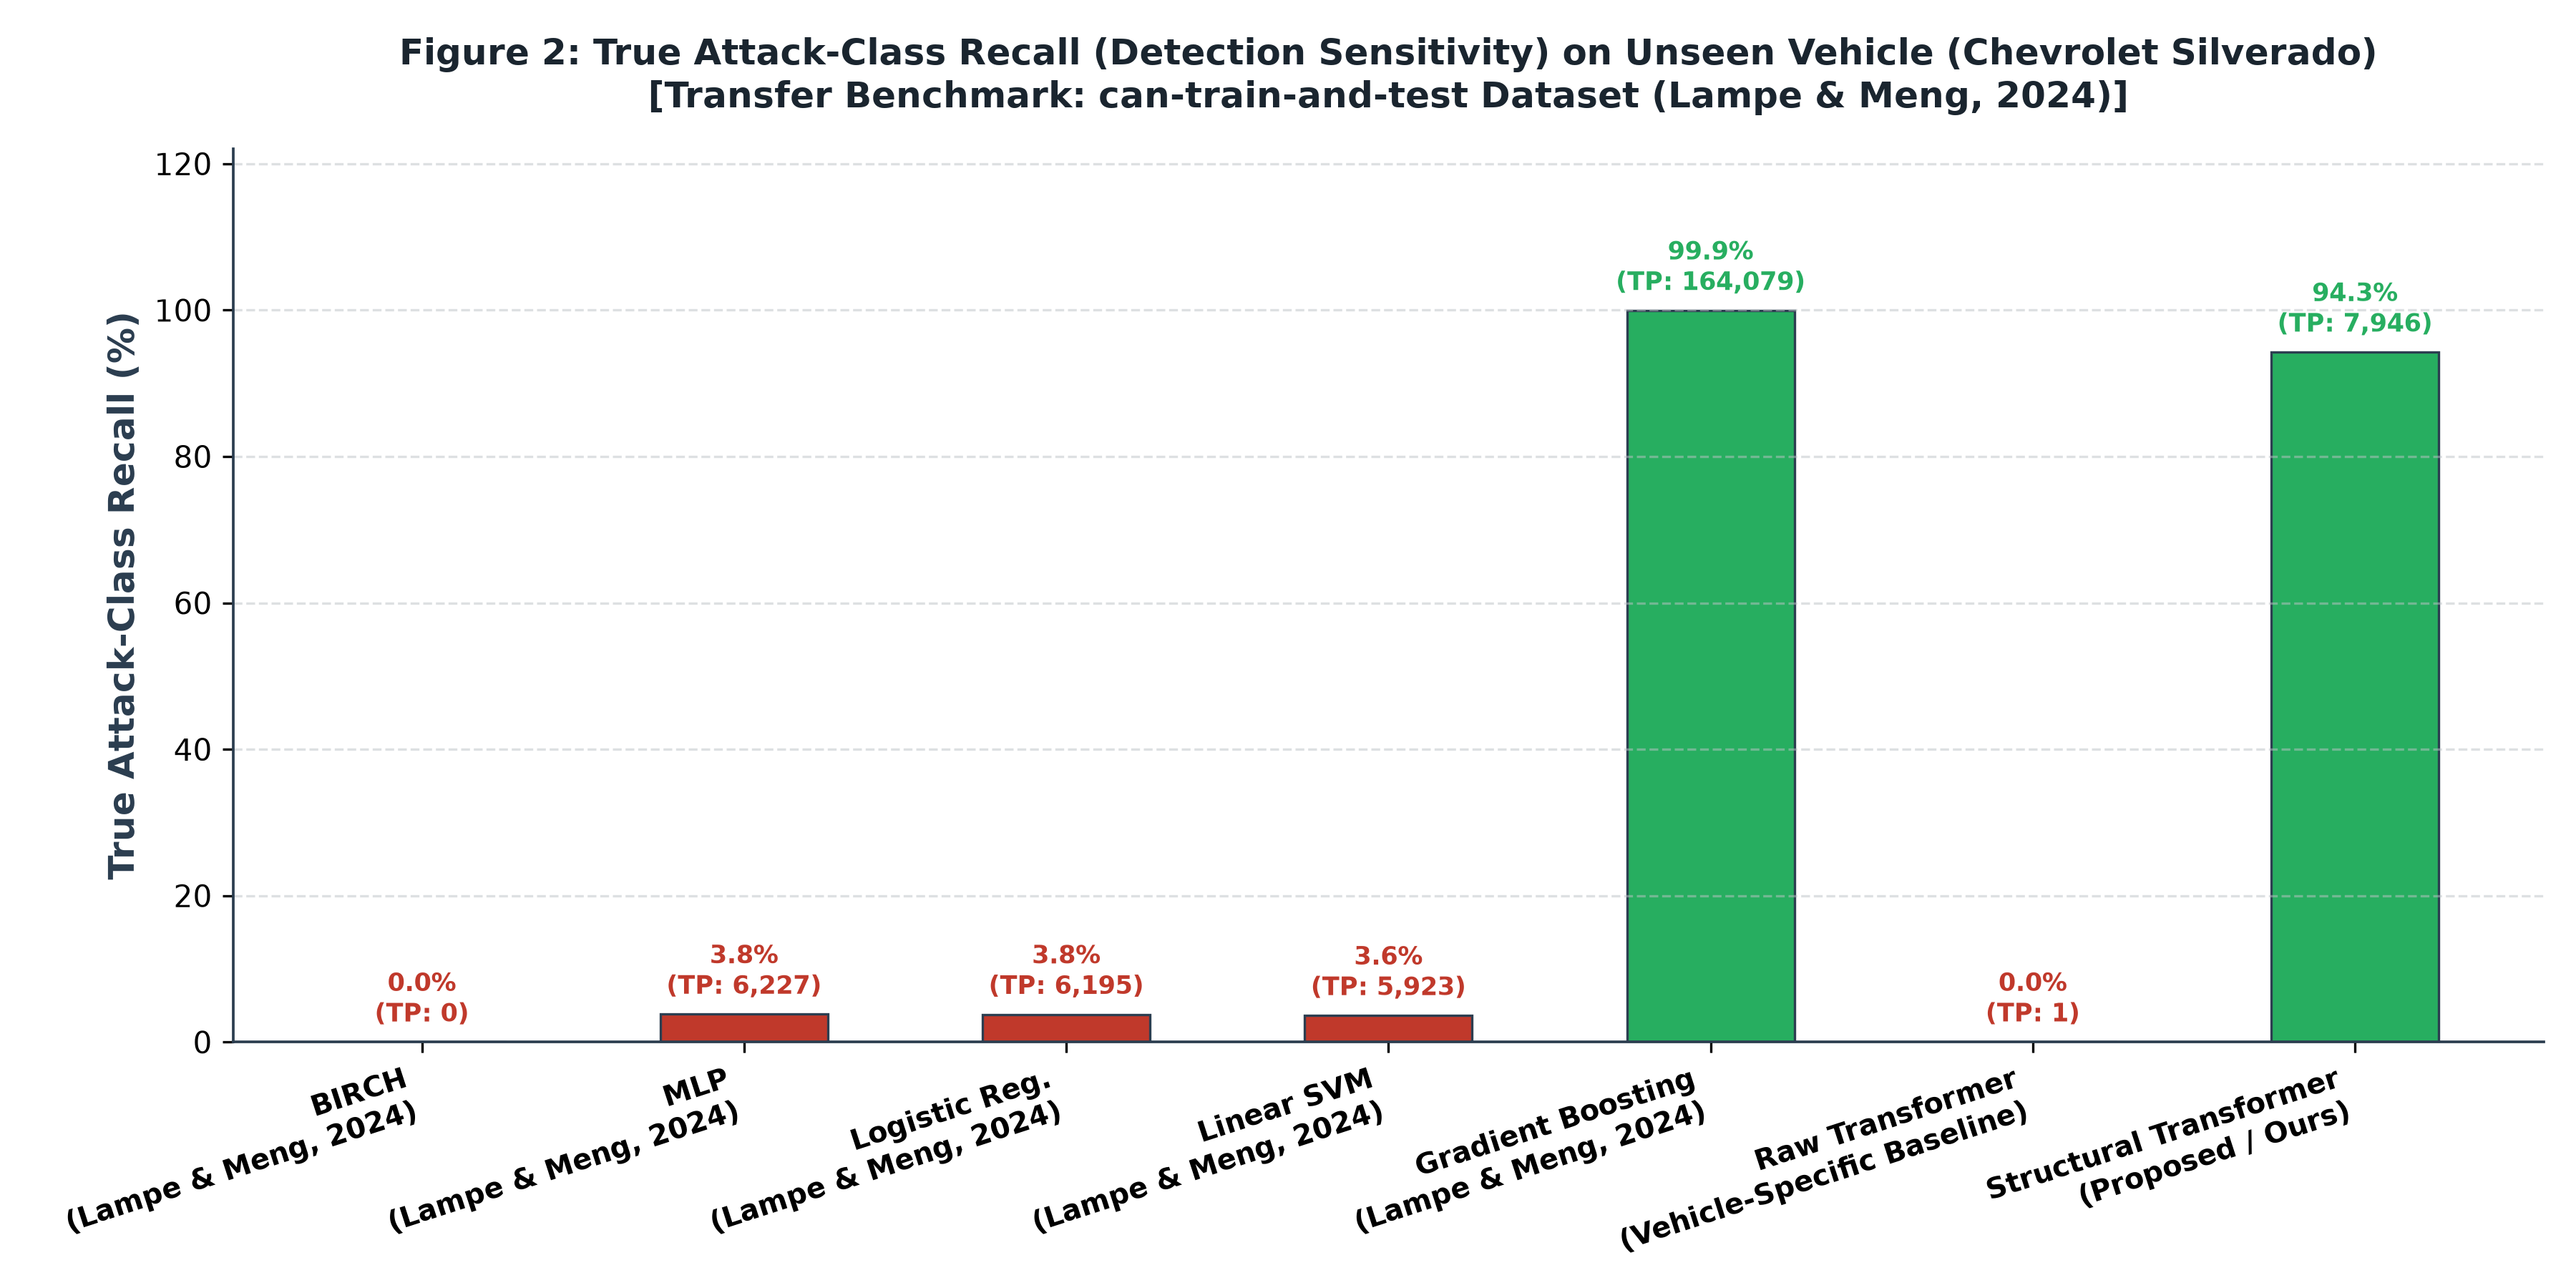
\includegraphics[width=\textwidth]{comparison_attack_recall.png}
\caption{Attack-class recall on the unseen Chevrolet Silverado transfer task, comparing published baselines with the two Transformer models.}
\label{fig:attack_recall}
\end{figure}

\section{External Validation}
\label{sec:external_validation}
Table~\ref{tab:external_results} summarizes representative rows from the external validation export. Results are heterogeneous. On selected CICIoV2024 DoS and GAS spoofing subsets, all three models attain F1 1.0, indicating that these scenarios are comparatively separable under the chosen windows. On Opel Astra and Renault Clio DoS files, the raw Transformer has near-perfect F1 while the structural Transformer falls to 0.3052 and 0.4409. On OTIDS, structural F1 remains 1.0 for DoS, falls to 0.7403 for fuzzy attacks, and falls sharply to 0.0906 for impersonation, compared with 1.0 for the raw Transformer. This is consistent with a boundary of the current representation: structural context transfers in some scenarios, but signal-level or protocol-specific cues can favor raw features.

\begin{table}[htbp]
\centering
\caption{Selected external validation results from the Phase~4 export}
\label{tab:external_results}
\small
\renewcommand{\arraystretch}{1.1}
\begin{tabular}{p{3.6cm}p{3.8cm}rr}
\hline
\textbf{Dataset and scenario} & \textbf{Model} & \textbf{Attack F1} & \textbf{FAR/100k} \\
\hline
OTIDS DoS & Raw Transformer & 1.0000 & 0.00 \\
OTIDS DoS & Structural Transformer & 1.0000 & 0.00 \\
OTIDS Fuzzy & Raw Transformer & 0.9952 & 0.00 \\
OTIDS Fuzzy & Structural Transformer & 0.7403 & 0.00 \\
OTIDS Impersonation & Raw Transformer & 1.0000 & 0.00 \\
OTIDS Impersonation & Structural Transformer & 0.0906 & 0.00 \\
Automotive v2, Opel Astra DoS & Raw Transformer & 1.0000 & 0.00 \\
Automotive v2, Opel Astra DoS & Structural Transformer & 0.3052 & 0.00 \\
Automotive v2, Renault Clio DoS & Raw Transformer & 0.9984 & 0.00 \\
Automotive v2, Renault Clio DoS & Structural Transformer & 0.4409 & 0.00 \\
CICIoV2024 DoS / GAS spoofing & Structural Transformer & 1.0000 & 0.00 \\
\hline
\end{tabular}
\end{table}

External false-alarm checks also show dataset sensitivity. On the OTIDS benign-driving subset, the raw Transformer records 100,000 false alarms per 100,000 benign windows, compared with 38,880 for the structural Transformer and 90 for structural XGBoost. The structural Transformer improves substantially over the raw baseline but still produces an unusably high alert burden in this test. The export reports zero FAR for the selected CICIoV2024 benign subset and selected CAN-MIRGU benign trace for the structural models, while the raw baseline reaches 100,000 in each. These checks are limited to selected files and do not establish robust operating thresholds across a full dataset.

The external notebook is an experimental validation pipeline rather than a harmonized benchmark. The available result table does not fully document per-file window counts, model checkpoint provenance, or a common calibration protocol for every external dataset. It also contains both attack and benign-only scenarios, which cannot share a single attack F1 interpretation. Results are therefore scenario-level observations, not a pooled estimate of generalization.

\begin{figure}[htbp]
\centering
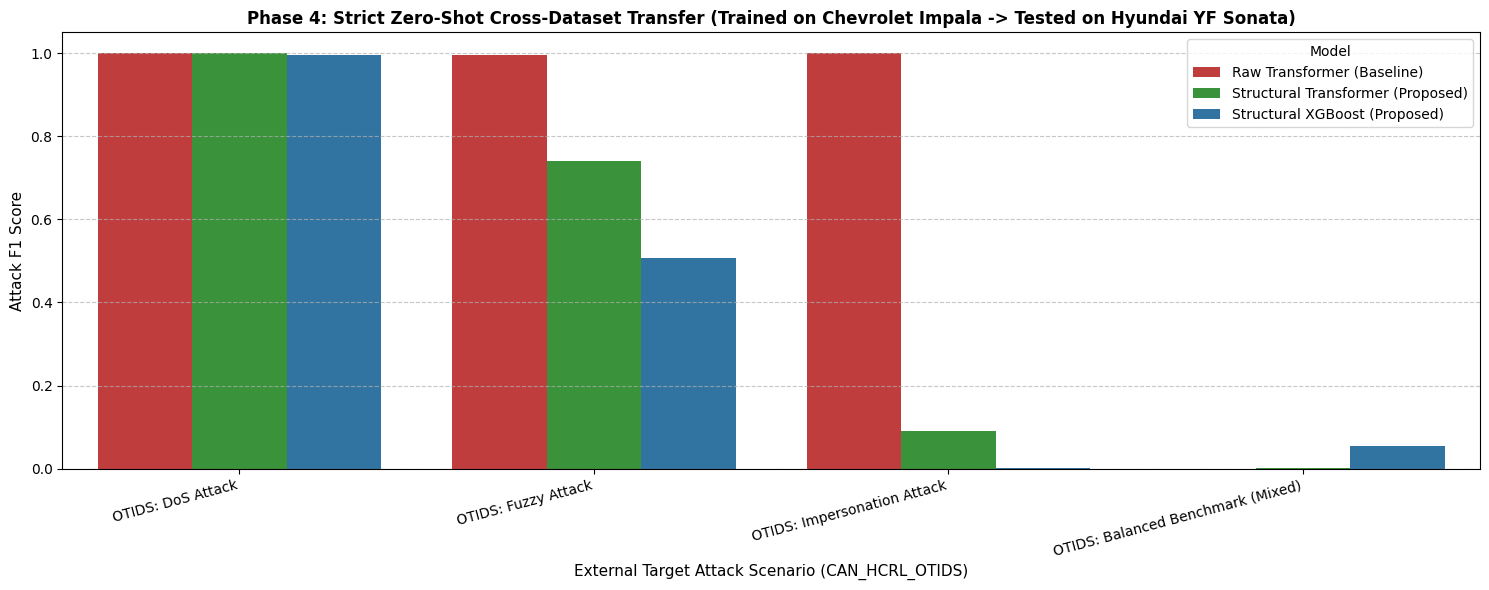
\includegraphics[width=\textwidth]{phase4_external_validation.png}
\caption{Attack F1 for selected OTIDS scenarios in the external validation export.}
\label{fig:otids_external}
\end{figure}

\section{Discussion}
\label{sec:discussion}
Three findings emerge. First, removing raw CAN-ID bits coincides with a large gain in Condition B for the focused experiment, where the attack family is known but the vehicle is unseen. The structural representation appears to preserve useful timing and within-window relational cues when the global ID vocabulary changes. Second, attack shift is harder than vehicle shift in the focused run: Condition C falls to F1 0.7094 and Condition D to 0.2332. The low D recall shows that high precision and a low false-alarm count can coexist with missed attacks. Third, external results are attack dependent. DoS detection transfers well in some datasets, while OTIDS impersonation and Automotive v2 DoS results favor the raw Transformer. A vehicle-agnostic representation is therefore not automatically attack-agnostic.

The focused Condition D result exceeds the predeclared three-point F1 improvement threshold over the raw Transformer, and Condition A does not decline. However, the success-gate CSV records only two gates, and the available artifacts do not provide paired bootstrap intervals or a complete vehicle-probe analysis. Thus, the results establish descriptive improvement in this run, not statistical significance or satisfaction of every criterion in the original project plan. The difference between focused and exploratory Set~1 exports reinforces the need for a frozen and reproducible evaluation pipeline before broad claims are made.



\chap{Conclusion and Future Work}
\label{chap:conclusions}
\sect{Main Contributions}

This thesis examined whether structural CAN traffic features can improve zero-shot intrusion detection across vehicles. On the focused \texttt{can-train-and-test} Set~1 experiment, the structural Transformer outperformed the raw-feature Transformer in all four reported conditions. The largest gain appeared in Condition B, where attack F1 increased from 0.0002 to 0.9703 for transfer to an unseen vehicle with known attacks. The method also improved Conditions C and D, although the D score of 0.2332 and recall of 0.1322 remain inadequate for dependable detection under simultaneous vehicle and attack shifts.

The thesis documented a 32-dimensional representation that replaces raw identifier bits with local identifier statistics while retaining payload, timing, and payload-change information. The controlled Transformer comparison suggests that both representation and sequence modeling matter: structural XGBoost did not match the structural Transformer under novel-attack conditions. External experiments revealed a mixed transfer picture, with excellent DoS results in some subsets and severe degradation on impersonation and selected cross-dataset DoS scenarios. These results support structural features as a useful direction for cross-vehicle CAN IDS, while limiting the claim to the evaluated experiments.



\sect{Limitations}

Several limitations constrain the conclusions. The main model comparison is based on a focused run from one benchmark set, and the four-set exploratory export contains materially different Set~1 scores. The available notebooks and CSV files do not provide a single end-to-end run manifest linking every metric to exact input files, checkpoints, software versions, and random seeds. No capture-group bootstrap confidence intervals are available, so uncertainty and statistical significance cannot be assessed. The feature extractor and training procedure also need a stricter audit of state at file and window boundaries to ensure identical causal context across implementations.

External validation covers selected files and attack scenarios rather than complete, harmonized datasets. Dataset label conventions, logging formats, and attack compositions differ, while current result exports do not consistently record sample counts and checkpoint provenance. Some benign false-alarm results are extremely high, and low FAR on a limited trace should not be read as a validated operational threshold. The study does not establish detection latency, runtime cost on an automotive platform, robustness to adaptive attackers, or performance after a vehicle firmware or driving-condition change. It also does not implement the planned feature-group ablation or a completed vehicle-probe study, so it cannot directly quantify how much vehicle information remains in the learned representation.



\sect{Future Works}

Future experiments should first freeze the data parser, feature extractor, split manifest, and training configuration, then rerun every benchmark set with saved checkpoints and per-file confusion matrices. A grouped bootstrap over captures or attack episodes should quantify uncertainty. The implementation should explicitly reset or carry causal feature state according to a documented rule at source-file and window boundaries, and automated checks should verify invariance under within-window identifier permutation.

The next model study should complete the planned ablations for raw ID, payload, timing, local structural features, and their combinations, while matching model capacity and training budgets. Vehicle-leakage probes can determine whether structural embeddings still reveal the source vehicle. Further work should evaluate threshold selection using source-only validation data, report recall at fixed false-alarm budgets, and measure event-level latency rather than only window-level classification. External validation should use complete and independently labeled traces from CAN-MIRGU, CICIoV2024, Automotive CAN v2, and OTIDS, with schema compatibility and file counts reported explicitly. Finally, attacks that preserve message order or timing, especially signal-level impersonation and replay, warrant dedicated features or complementary detectors.


\newpage
\addcontentsline{toc}{chapter}{Bibliography} 
% \bibliographystyle{plainnat}
\bibliographystyle{ieeetr}
\bibliography{refs}

\end{document}
